%
% geradeaxb.tex
%
% (c) 2018 Prof Dr Andreas Müller, Hochschule Rapperswil
%
\documentclass[tikz,12pt]{standalone}
\usepackage{times}
\usepackage{amsmath}
\usepackage{txfonts}
\usepackage[utf8]{inputenc}
\usepackage{graphics}
\usepackage{color}
\usepackage{pifont}
\usetikzlibrary{arrows,intersections,math,calc}
\begin{document}

\def\punkt#1{
        \fill[color=white] #1 circle[radius=0.08];
        \draw #1 circle[radius=0.08];
}

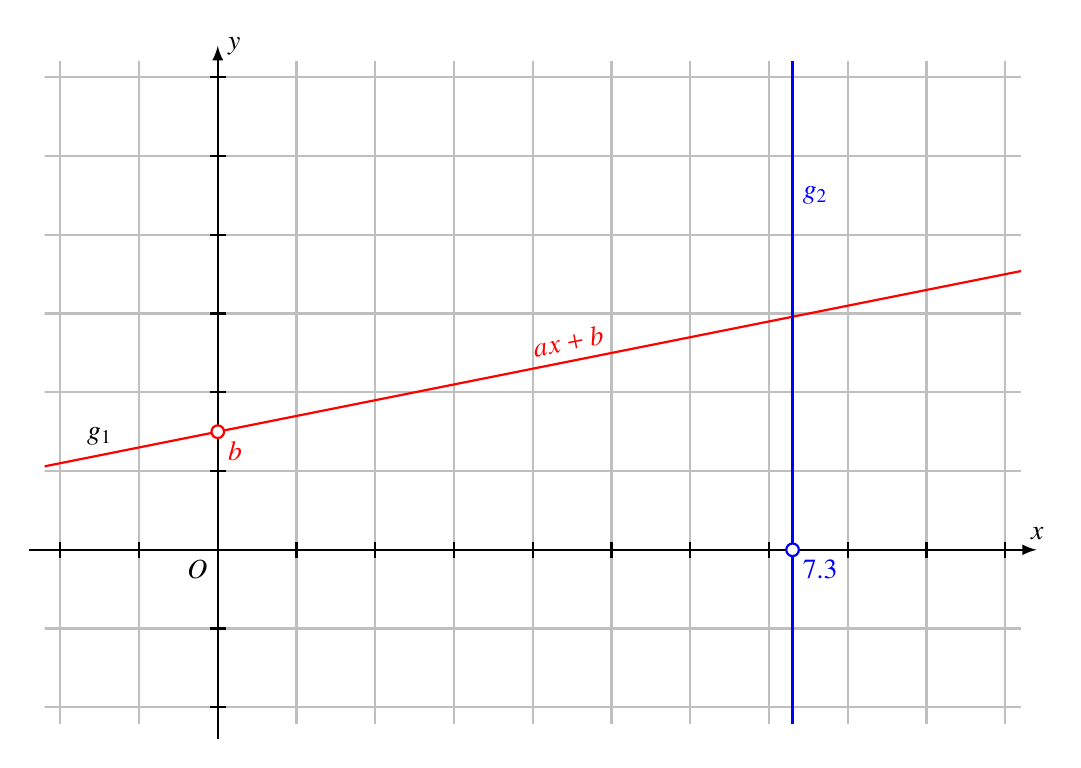
\begin{tikzpicture}[>=latex,thick]

% coordinate 
\begin{scope}
\clip (-2.2,-2.2) rectangle (10.2,6.2);
\foreach \x in {-2,-1,...,10}{
	\draw[color=gray!50] (\x,-10)--(\x,10);
	\draw (\x,-0.1)--(\x,0.1);
%	\node at (\x,0) [below right] {$\x$};
}
\foreach \y in {-2,-1,...,6}{
	\draw[color=gray!50] (-10,\y)--(20,\y);
	\draw (-0.1,\y)--(0.1,\y);
}
\end{scope}

% coordinate axes
\draw[->] (-2.4,0)--(10.4,0) coordinate[label=$x$];
\draw[->] (0,-2.4)--(0,6.4) coordinate[label={right:$y$}];

% Origin
\punkt{(0,0)}
\node at (0,0) [below left] {$O$};

% Geraden
\begin{scope}
\clip (-2.2,-2.2) rectangle (10.2,6.2);
\draw[color=red] (-8,{1.5 + 0.2*(-8)})--(18,{1.5 + 0.2*18});
\end{scope}

\fill[color=white] (0,1.5) circle[radius=0.08];
\draw[color=red] (0,1.5) circle[radius=0.08];
\node[color=red] at (0,1.5) [below right] {$b$};
\node[color=red] at (4.5,{1.5+0.2*4.5}) [above,rotate={atan(0.2)}] {$ax+b$};

\node at (-1.5,{1.5-0.2*1.5}) [above] {$g_1$};

% Verticale Gerade
\def\xx{7.3}
\begin{scope}
\clip (-2.2,-2.2) rectangle (10.2,6.2);
\draw[color=blue] (\xx,-10)--(\xx,10);
\end{scope}
\fill[color=white] (\xx,0) circle[radius=0.08];
\draw[color=blue] (\xx,0) circle[radius=0.08];
\node[color=blue] at (\xx,0) [below right] {$\xx$};

\node[color=blue] at (\xx,4.5) [right] {$g_2$};

\end{tikzpicture}

\end{document}

